\chapter{Long Term Evolution}

\section{Communication Systems Overview}

\section{Digital Communications Overview}
\label{sec:digitalcomm}

\subsection{Synchronization}

\subsubsection{Carrier Recovery}

Carrier recovery is a process used in coherent demodulation where the phase
and the frequency of the transmitter carrier wave are recovered by the receiver
and thus after having such information it is possible to extract the information
in the transmitted signal.\\
Considering that the phase and frequency of the transmitted wave probably will
be affected by noise, it is not a straight-forward method, it includes filtering
and usually feedback systems to correct the erros in phase or frequency caused
by the noise.\\
This chapter aims in the brief exploration of some techniques used for carrier
recovering, such as Phase locked loops, costas loop and others.\\

\subsubsection{Costas Loop}


\section{Long Term Evolution}

\subsection{Overview}

Long Term Evolution (LTE) is a standard for wireless communication for high-speed
mobile devices and data terminals. LTE was first introduced in 3GPP Release 8.
It uses orthogonal frequency division multiplexing (OFDM) as its radio access
technology, together with advanced antenna technologies.\\

In addition to LTE, 3GPP also defined IP-based, flat core network architecture.
This architecture was defined as part of the System Architecture Evolution (SAE)
effort specifying the Evolved Packet Core (EPC) network. The LTE-SAE architecture
and concepts have been designed for efficient support of mass-market usage of any
IP-based service. The architecture is based on an evolution of the existing GSM/WCDMA
core network, with simplified operations and smooth, cost-efficient deployment.\\

Moreover, work has also been done by 3GPP in cooperation with 3GPP2 (the CDMA
standardization body) to optimize interworking between CDMA and LTE-SAE. This means
that both CDMA and GSM operators can use the same standard with minor modifications
and thus making the deployment and roaming costs smaller.\\

LTE can be was thought to reduce cost in deployment in legacy systems, as said
before with CDMA and GSM, it can use the legacy systems and adapt itself to work
with them, creating a smooth transition for the network operators \cite{introlte}.\\

The 3GPP radio access  technology was developed towards:

\begin{itemize}
    \item Reduced cost per bit
    \item Increased service provisioning – more services at a lower cost with
    better user experience
    \item Flexible use of existing and new frequency bands
    \item Simplified architecture and open interfaces
    \item Reasonable terminal power consumption
\end{itemize}

The specification work on LTE was completed in March 2009 as the SAE specifications
were included. Below it is possible to see some of the 3GPP Release 8 LTE Requirements:

\begin{itemize}
    \item Increased peak data rates: 100Mbps downlink and 50Mbps uplink
    \item Reduction of Radio Access Network (RAN) latency to 10ms
    \item Improved spectrum efficiency (two to four times compared with HSPA Release 6)
    \item Cost-effective migration from Release 6 Universal Terrestrial Radio
    Access (UTRA) radio interface and architecture
    \item Improved broadcasting
    \item IP-optimized (focus on services in the packet switched domain)
    \item Scalable bandwidth of 20MHz, 15MHz, 10MHz, 5MHz, 3MHz and 1.4MHz
    \item Support for both paired and unpaired spectrum
    \item Support for interworking with existing 3G systems and non-3GPP specified systems.
\end{itemize}

\subsection{Network Architecture}

In parallel with the LTE radio access, the packet core network was implemented as
flat IP-based multi-access core network. The Evolved Packet Core (EPC) network was
designed to optimize network performance, improve cost-efficiency and facilitate
the uptake of mass-market multimedia services.\\

Existing 3GPP (GSM and WCDMA/HSPA) and 3GPP2 (CDMA2000 1xRTT, EV-DO) systems are
integrated to the EPC network through standardized interfaces providing optimized
mobility with LTE. For 3GPP systems this means a signaling interface between the
existing Serving GPRS Support Node (SGSN) to the Mobility Management Entity (MME)
in the EPC network; for 3GPP2 a control signaling interface between the CDMA RAN
and the MME. This integration support both dual and single radio handover, allowing
a flexible migration to LTE.\\

The Home Subscriber Server (HSS) connects to the Packet Core through an IP-based
interface using Diameter, and not SS7, which was used in previous GSM and WCDMA
networks. Network signaling for policy control and charging is already based on
Diameter. This means that all interfaces in the new architecture are IP-based.\\

LTE-EPC has adopted an effective class-based QoS concept. This provides a
foundation for operators to offer service differentiation, depending on the type
of subscription or application.

%figura da rede
\begin{figure}[htbp]
    \centering
    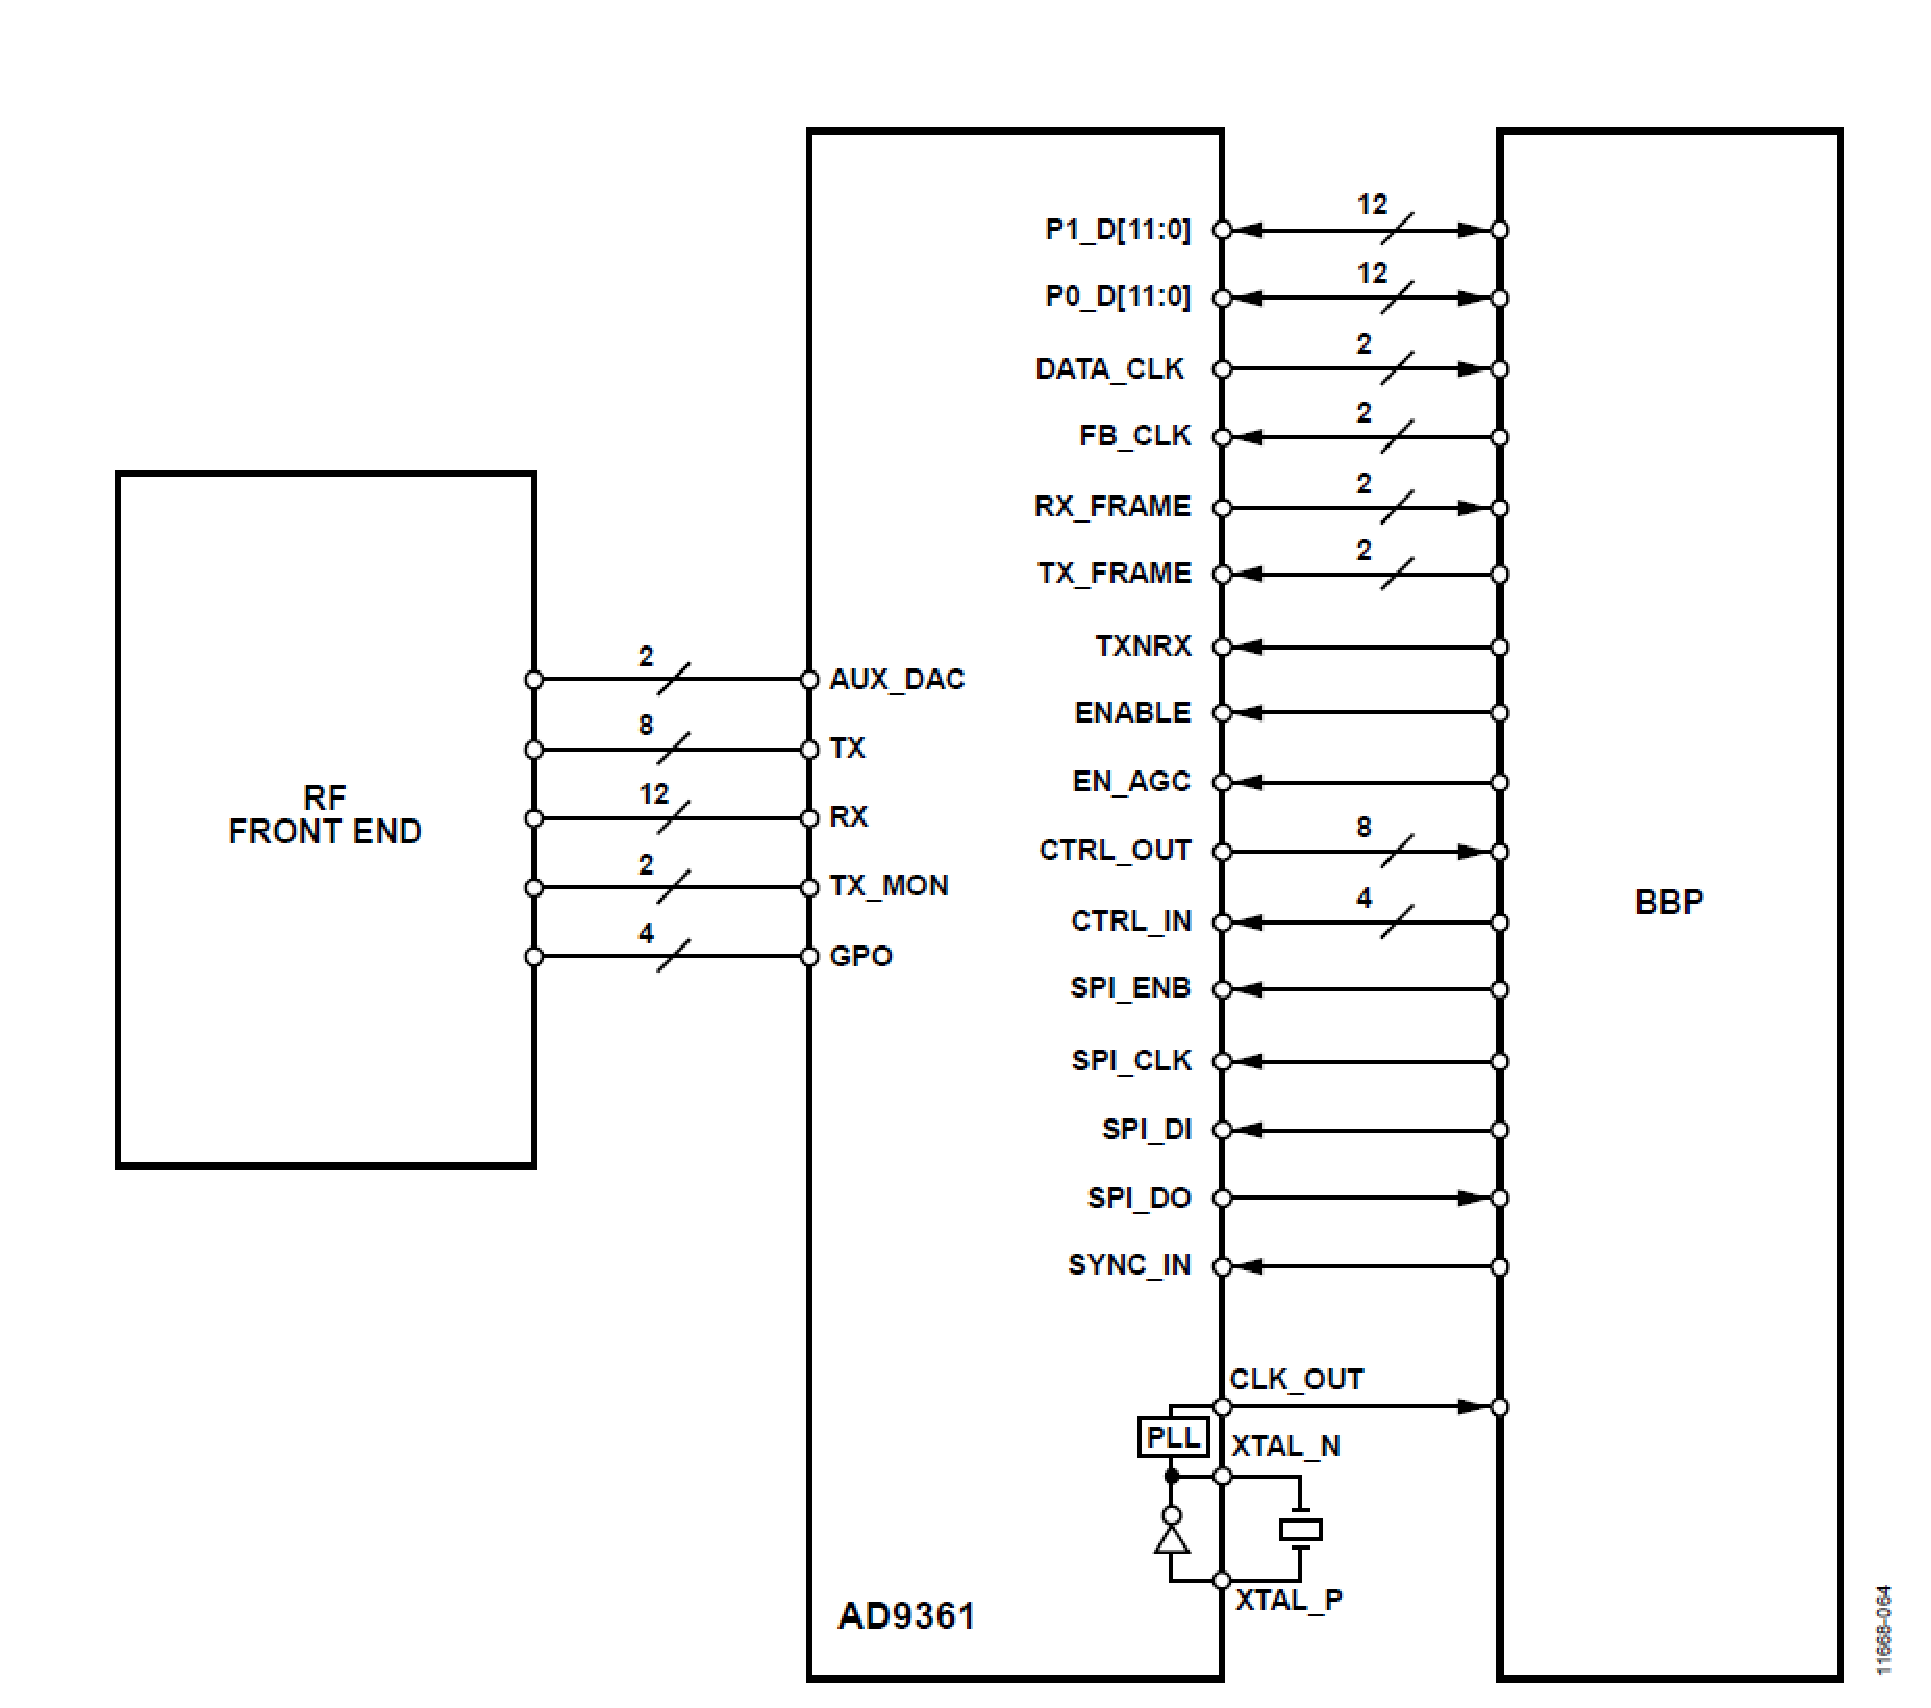
\includegraphics[width=0.65\textwidth]{./figures/ad9361_digital_interface}
    \caption{ AD9361 Digital Data Interface
    \label{fig:ad9361diginterface}}
\end{figure}

\subsection{Orthogonal Frequency-division Multiplexing Radio Technology}

LTE uses OFDM for the downlink ( from the base station to the terminal or UE).
OFDM meets the LTE requirement for spectrum flexibility and enables cost-efficient
solutions for very wide carriers with high peak rates. It is a well-established
technology: for example, in standards such as IEEE 802.11a/b/g, 802.16, HIPERLAN-2,
DVB and DAB.\cite{introlte} \cite{umtslte}\\

OFDM uses a large number of narrow sub-carriers for multi-carrier transmission.
The basic LTE downlink physical resource can be seen as a time-frequency grid.
In the frequency domain, the spacing between the sub-carriers, $\Delta f$, is 15
kHz. In addition, the OFDM symbol duration time is $\frac{1}{\Delta f} + cyclic prefix$.
The cyclic prefix is used to maintain orthogonality between the sub-carriers even
for a time-dispersive radio channel. One resource element carries QPSK, 16QAM or
64QAM. With 64QAM, each resource element carries six bits.\\

The OFDM symbols are grouped into resource blocks. The resource blocks have a
total size of 180 kHz in the frequency domain and 0.5ms in the time domain. Each
user is allocated a number of so-called resource blocks in the time-frequency grid.
The more resource blocks a user gets, and the higher the modulation used in the
resource elements, the higher the bit rate. Which resource blocks the user gets
at a given point in time, and how many, depends on advanced scheduling mechanisms
in the frequency and time dimensions.\\

Scheduling of resources can be taken every 1ms: that means two resource blocks,
180 kHz wide and in total 1ms in length (called a Scheduling Block). The scheduling
mechanisms in LTE are similar to those used in HSPA, and enable optimal performance
for different services in different radio environments.\\

In the uplink, LTE uses a pre-coded version of OFDM called Single Carrier Frequency
Division Multiple Access (SC-FDMA). This is to compensate for a drawback with normal
OFDM, which has a very high Peak to Average Power Ratio (PAPR). High PAPR requires
expensive and inefficient power amplifiers with high linearity requirements, which
increases the cost of the terminal and drains the battery faster.\\

SC-FDMA solves this problem by grouping together the resource blocks in such a
way that it reduces the need for linearity, and so power consumption, in the
power amplifier. A low PAPR also improves coverage and cell-edge performance.

Since this work shall focus on the Radio Frontend part of the systems, implementing
a downlink scheme, it is interesting to dwell more in the LTE downlink and uplink
schemes.

\subsection{Downlink Scheme}

The downlink transmission scheme for E-UTRA FDD and TDD modes is based on
conventional OFDM. In an OFDM system, the available spectrum is divided into
multiple carriers, called subcarriers. Each of these subcarriers is independently
modulated by a low rate data stream. OFDM is used as well in WLAN, WiMAX and
broadcast technologies like DVB. OFDM has several benefits including its robustness
against multipath fading and its efficient receiver architecture.\\

Figure 2 shows a representation of an OFDM signal. In this figure, a signal with
5 MHz bandwidth is shown, but the principle is of course the same for the other
E-UTRA bandwidths. Data symbols are independently modulated and
transmitted over a high number of closely spaced orthogonal subcarriers.\\

In E-UTRA, downlink modulation schemes QPSK, 16QAM, and 64QAM are available.
In the time domain, a guard interval is added to each symbol to combat
inter-symbolinterference (ISI) due to channels delay spread. The delay spread is
the time between the symbol arriving on the first multi-path signal and the last
multi-path signal component, typically several $\mu s$ dependent on the environment
(i.e. indoor, rural, suburban, city center). The guard interval has to be selected
in that way, that it is greater than the maximum expected delay spread. In E-UTRA,
the guard interval is a cyclic prefix which is inserted prior to each OFDM symbol.

%figura ondas
\begin{figure}[htbp]
    \centering
    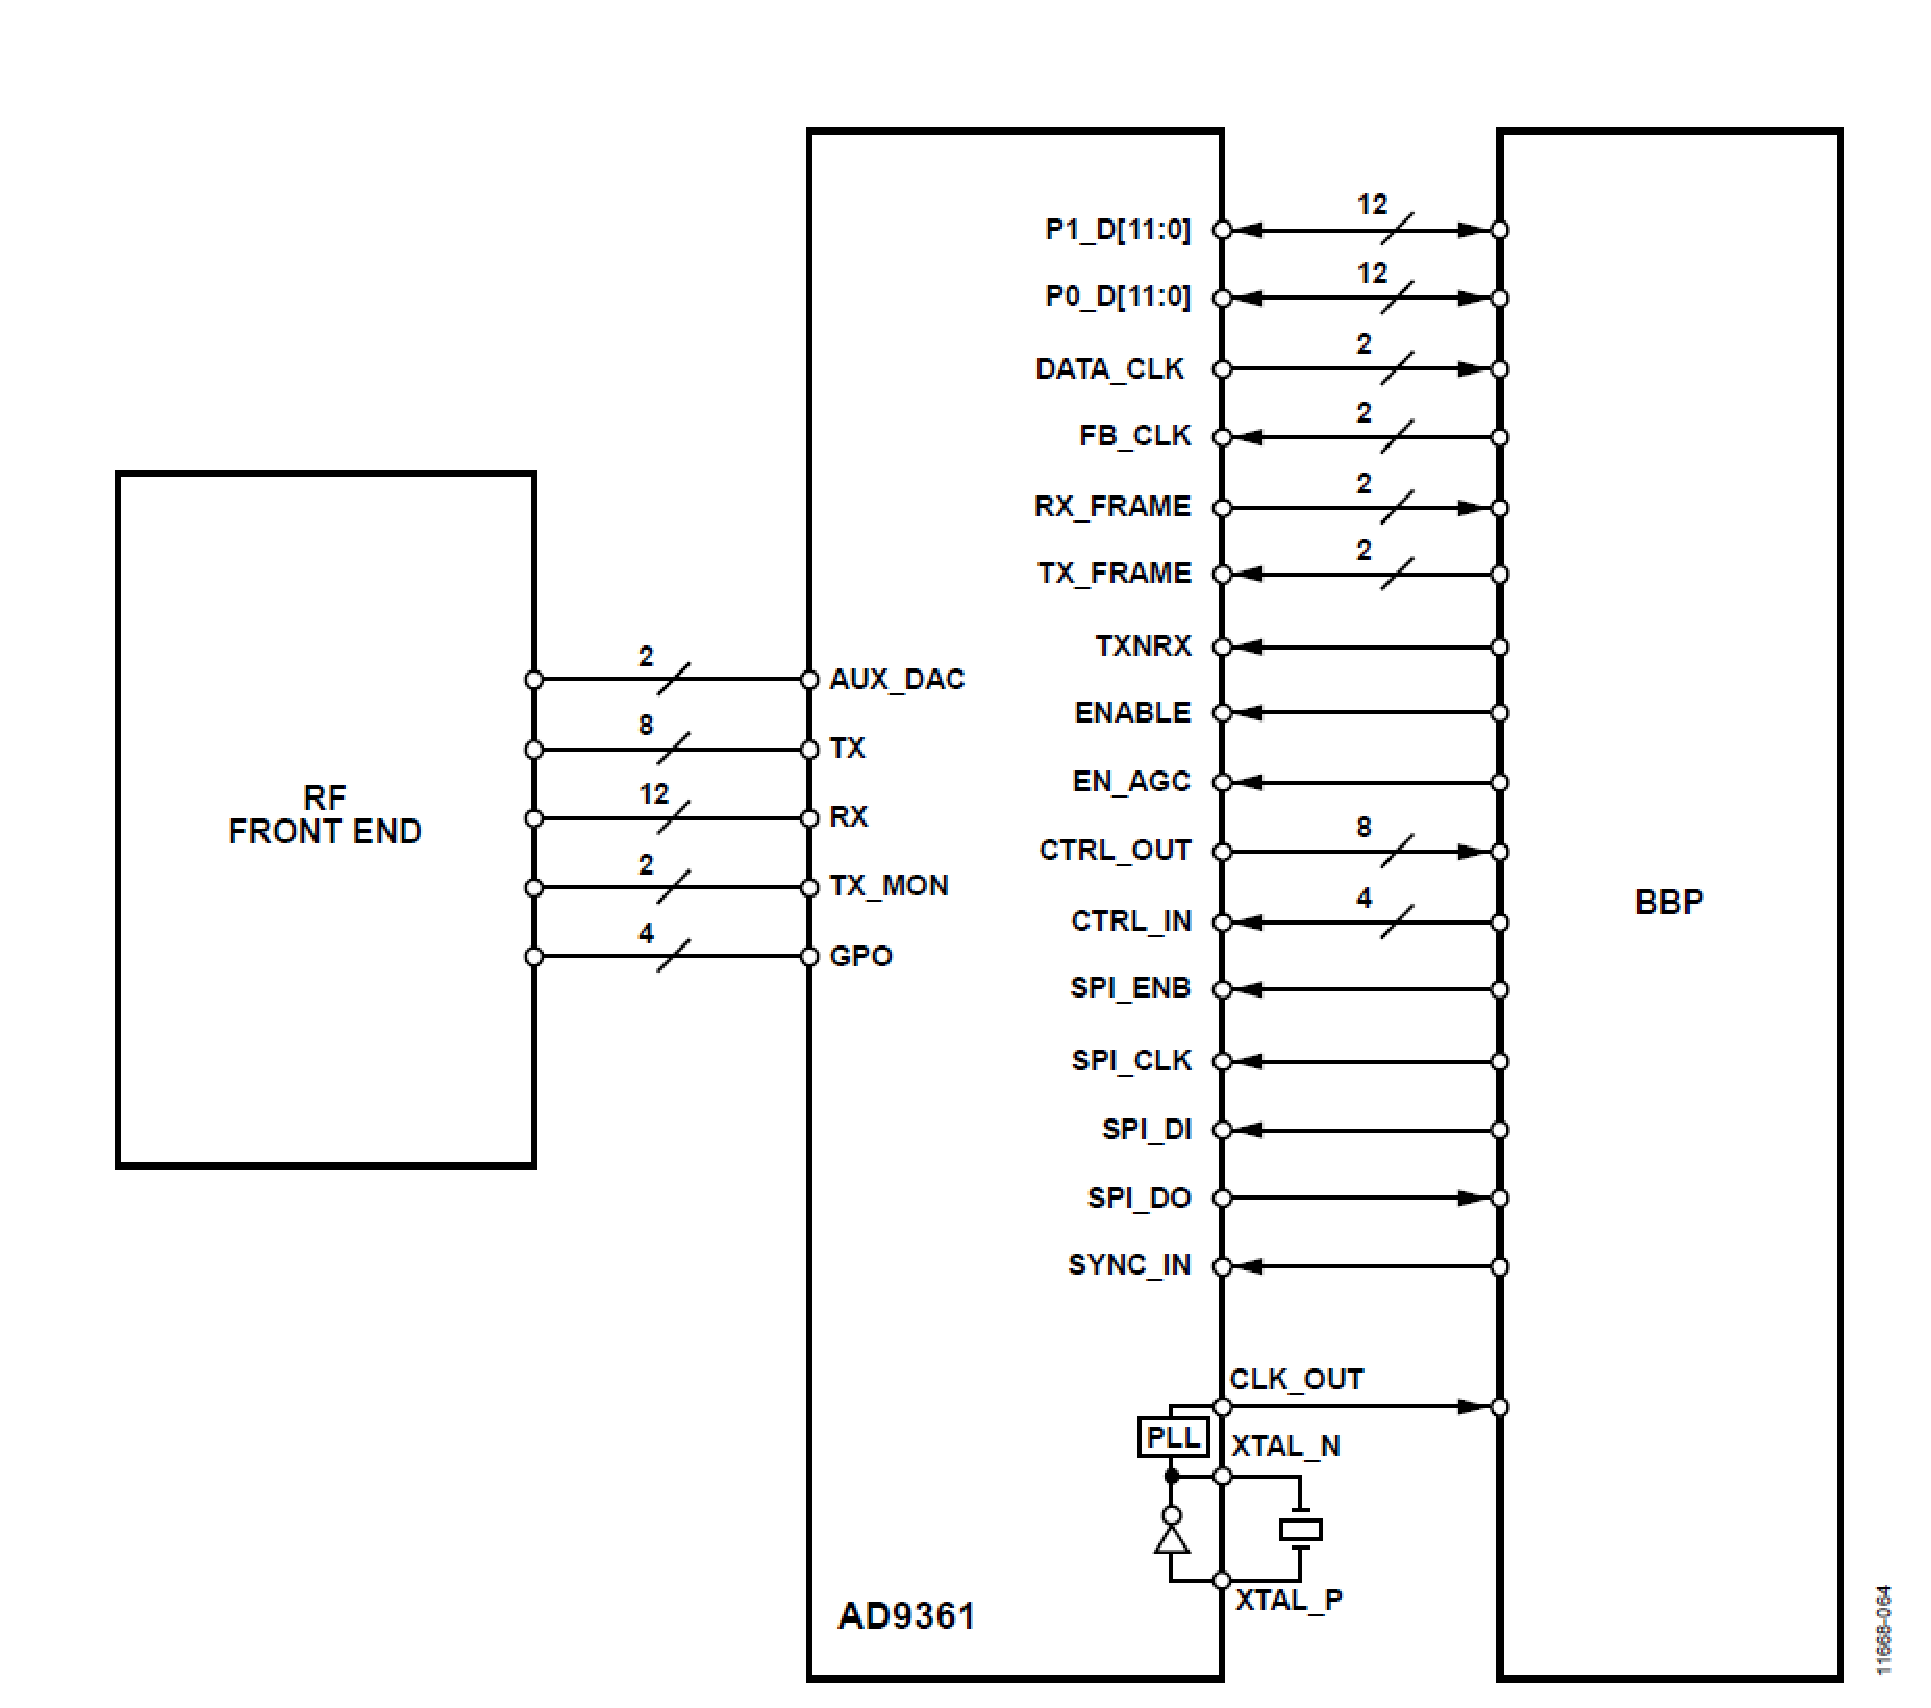
\includegraphics[width=0.65\textwidth]{./figures/ad9361_digital_interface}
    \caption{ AD9361 Digital Data Interface
    \label{fig:ad9361diginterface}}
\end{figure}

In practice, the OFDM signal can be generated using IFFT (Inverse Fast Fourier Transform)
digital signal processing. The IFFT converts a number N of complex data
symbols used as frequency domain bins into the time domain signal. Such an N-point
IFFT is illustrated in Figure X where $a(mN+n)$ refers to the nth subcarrier
modulated data symbol, during the time period $mTu < t £ (m+1)Tu$.

%figura esquema
\begin{figure}[htbp]
    \centering
    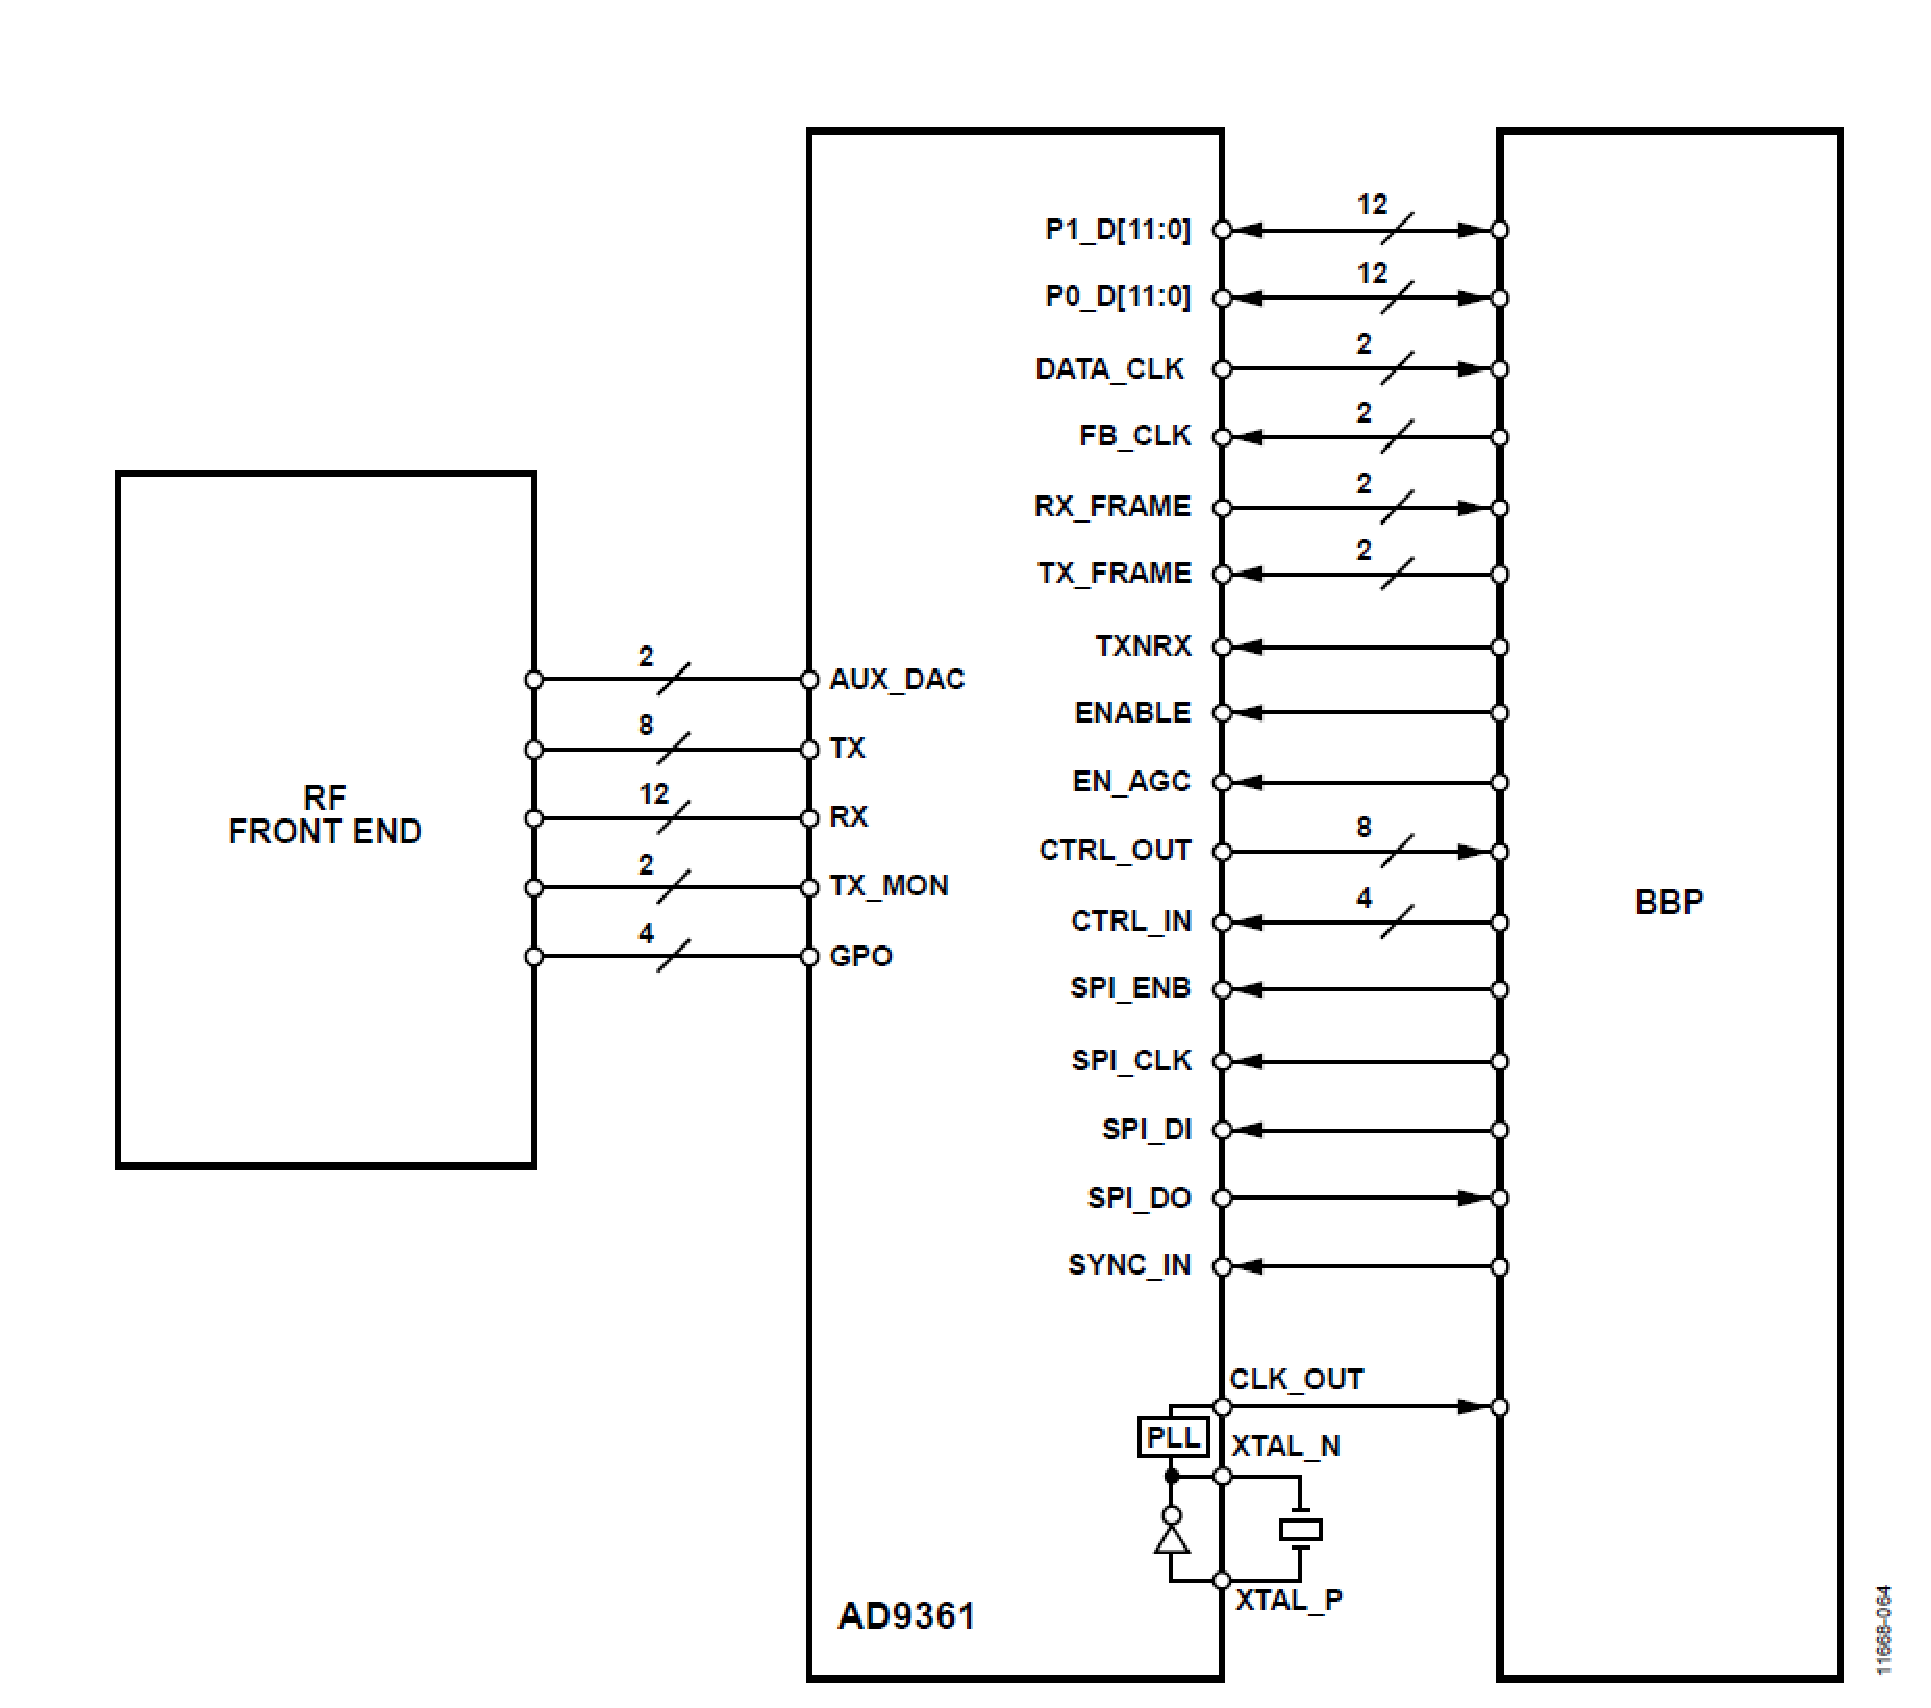
\includegraphics[width=0.65\textwidth]{./figures/ad9361_digital_interface}
    \caption{ AD9361 Digital Data Interface
    \label{fig:ad9361diginterface}}
\end{figure}


The vector $sm$ is defined as the useful OFDM symbol. It is the time superposition
of the $N$ narrowband modulated subcarriers. Therefore, from a parallel stream
of $N$ sources of data, each one independently modulated, a waveform composed of
N orthogonal subcarriers is obtained, with each subcarrier having the shape of a
frequency sinc function (see Figure 2). Figure 4 illustrates the mapping from a
serial stream of QAM symbols to N parallel streams, used as frequency domain bins
for the IFFT. The N-point time domain blocks obtained from the IFFT are then
serialized to create a time domain signal.

%figura signal generation

\begin{figure}[htbp]
    \centering
    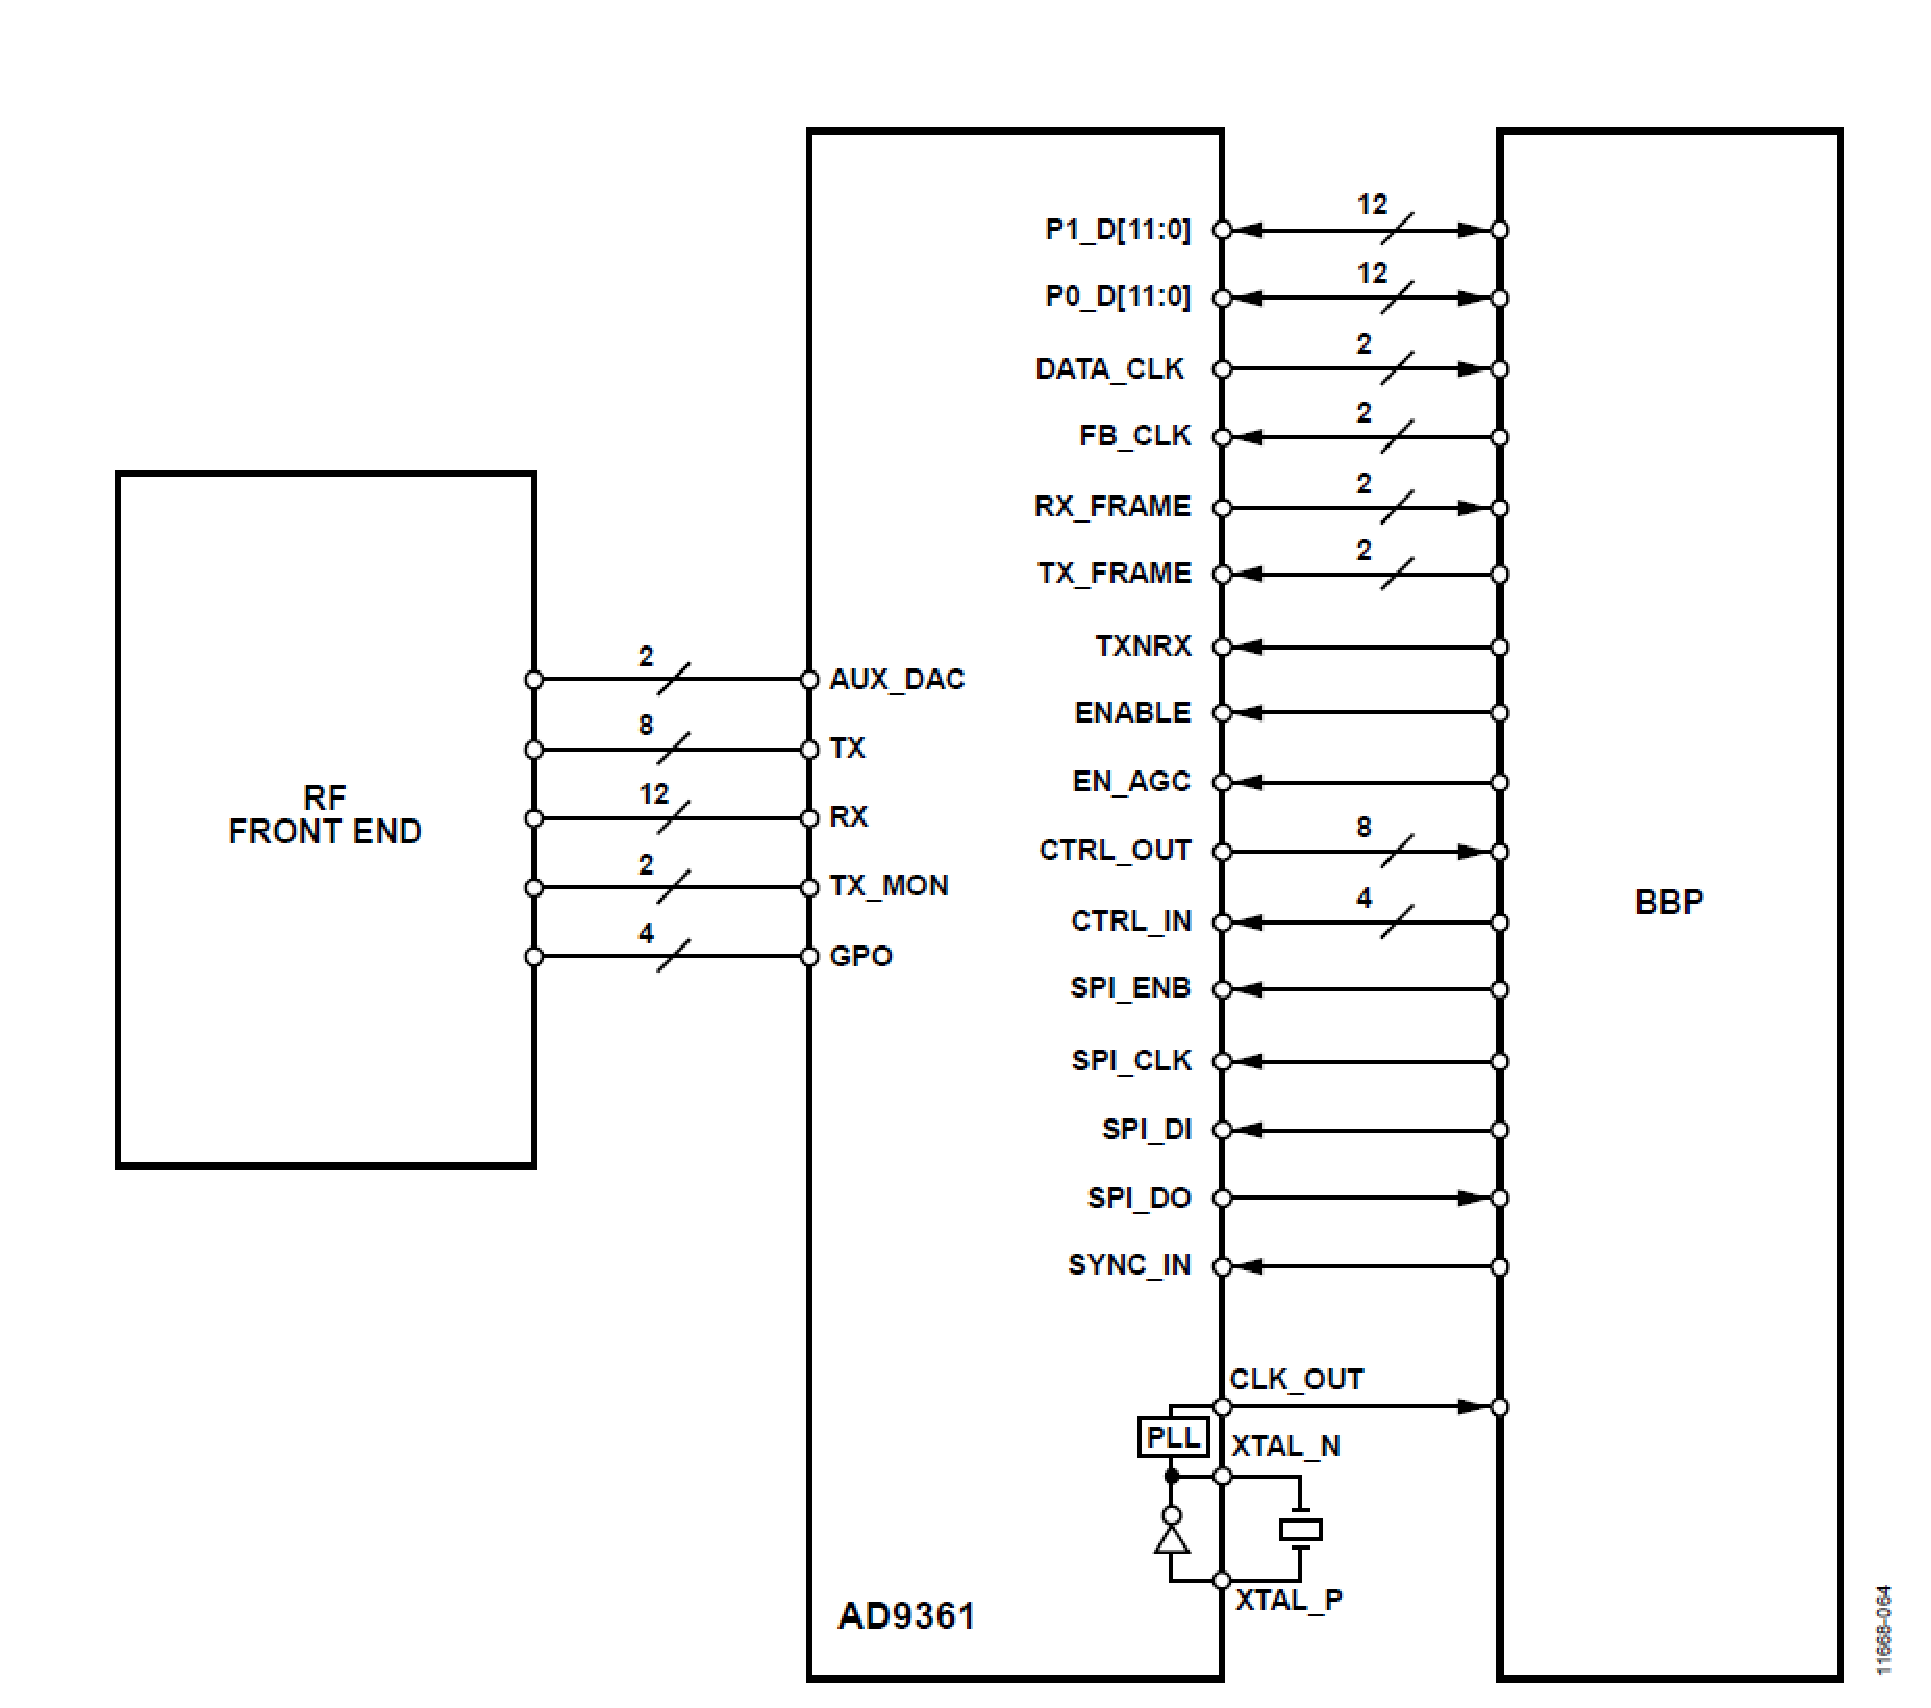
\includegraphics[width=0.65\textwidth]{./figures/ad9361_digital_interface}
    \caption{ AD9361 Digital Data Interface
    \label{fig:ad9361diginterface}}
\end{figure}

In contrast to an OFDM transmission scheme, OFDMA allows the access of multiple
users on the available bandwidth. Each user is assigned a specific time-frequency
resource.

As stated before the data is allocated to a device (User Equipment, UE) in terms
of resource blocks, i.e. one UE can be allocated integer multiples of one resource
block in the frequency domain. These resource blocks do not have to be adjacent to
each other. In the time domain, the scheduling decision can be modified every
transmission time interval of 1 ms. All scheduling decisions for downlink and
uplink are done in the base station (enhanced NodeB, eNodeB or eNB). The scheduling
algorithm has to take into account the radio link quality situation of different
users, the overall interference situation, Quality of Service requirements, service
priorities, etc. and is a vendor-specific implementation. Figure 8 shows an example
for allocating downlink user data to different users.\\


%figura resource block

\begin{figure}[htbp]
    \centering
    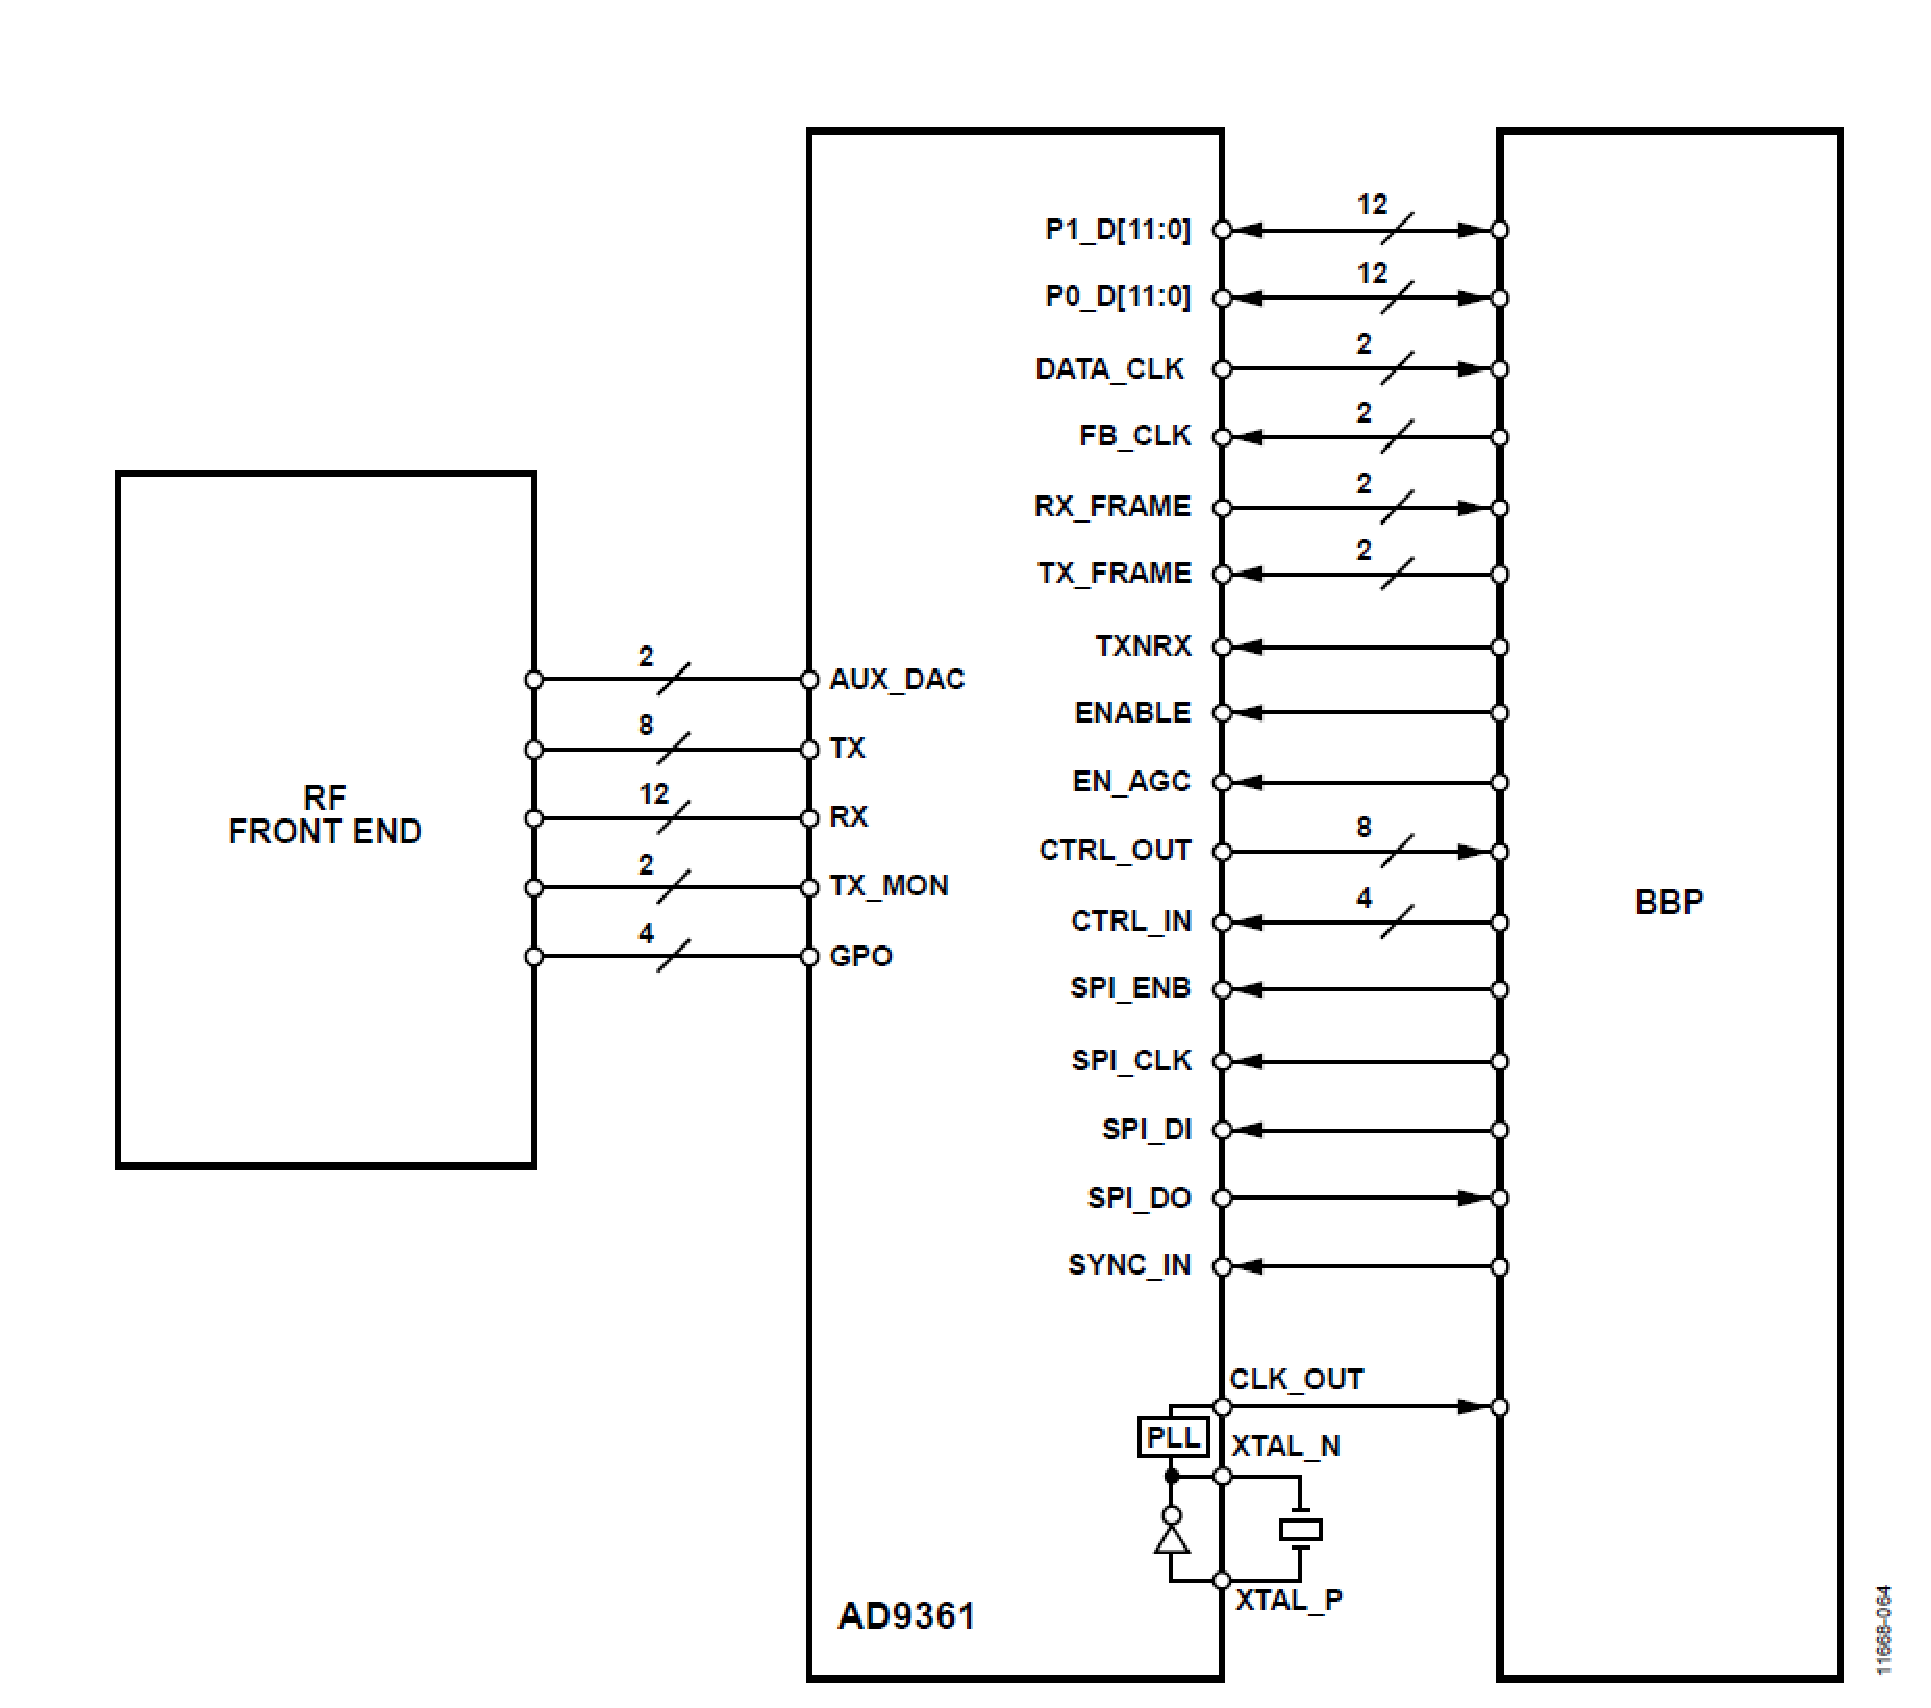
\includegraphics[width=0.65\textwidth]{./figures/ad9361_digital_interface}
    \caption{ AD9361 Digital Data Interface
    \label{fig:ad9361diginterface}}
\end{figure}

The user data is carried on the Physical Downlink Shared Channel (PDSCH). The
PDSCH(s) is the only channel that can be QPSK, 16QAM or 64QAM modulated.

%downlink channel figura
\begin{figure}[htbp]
    \centering
    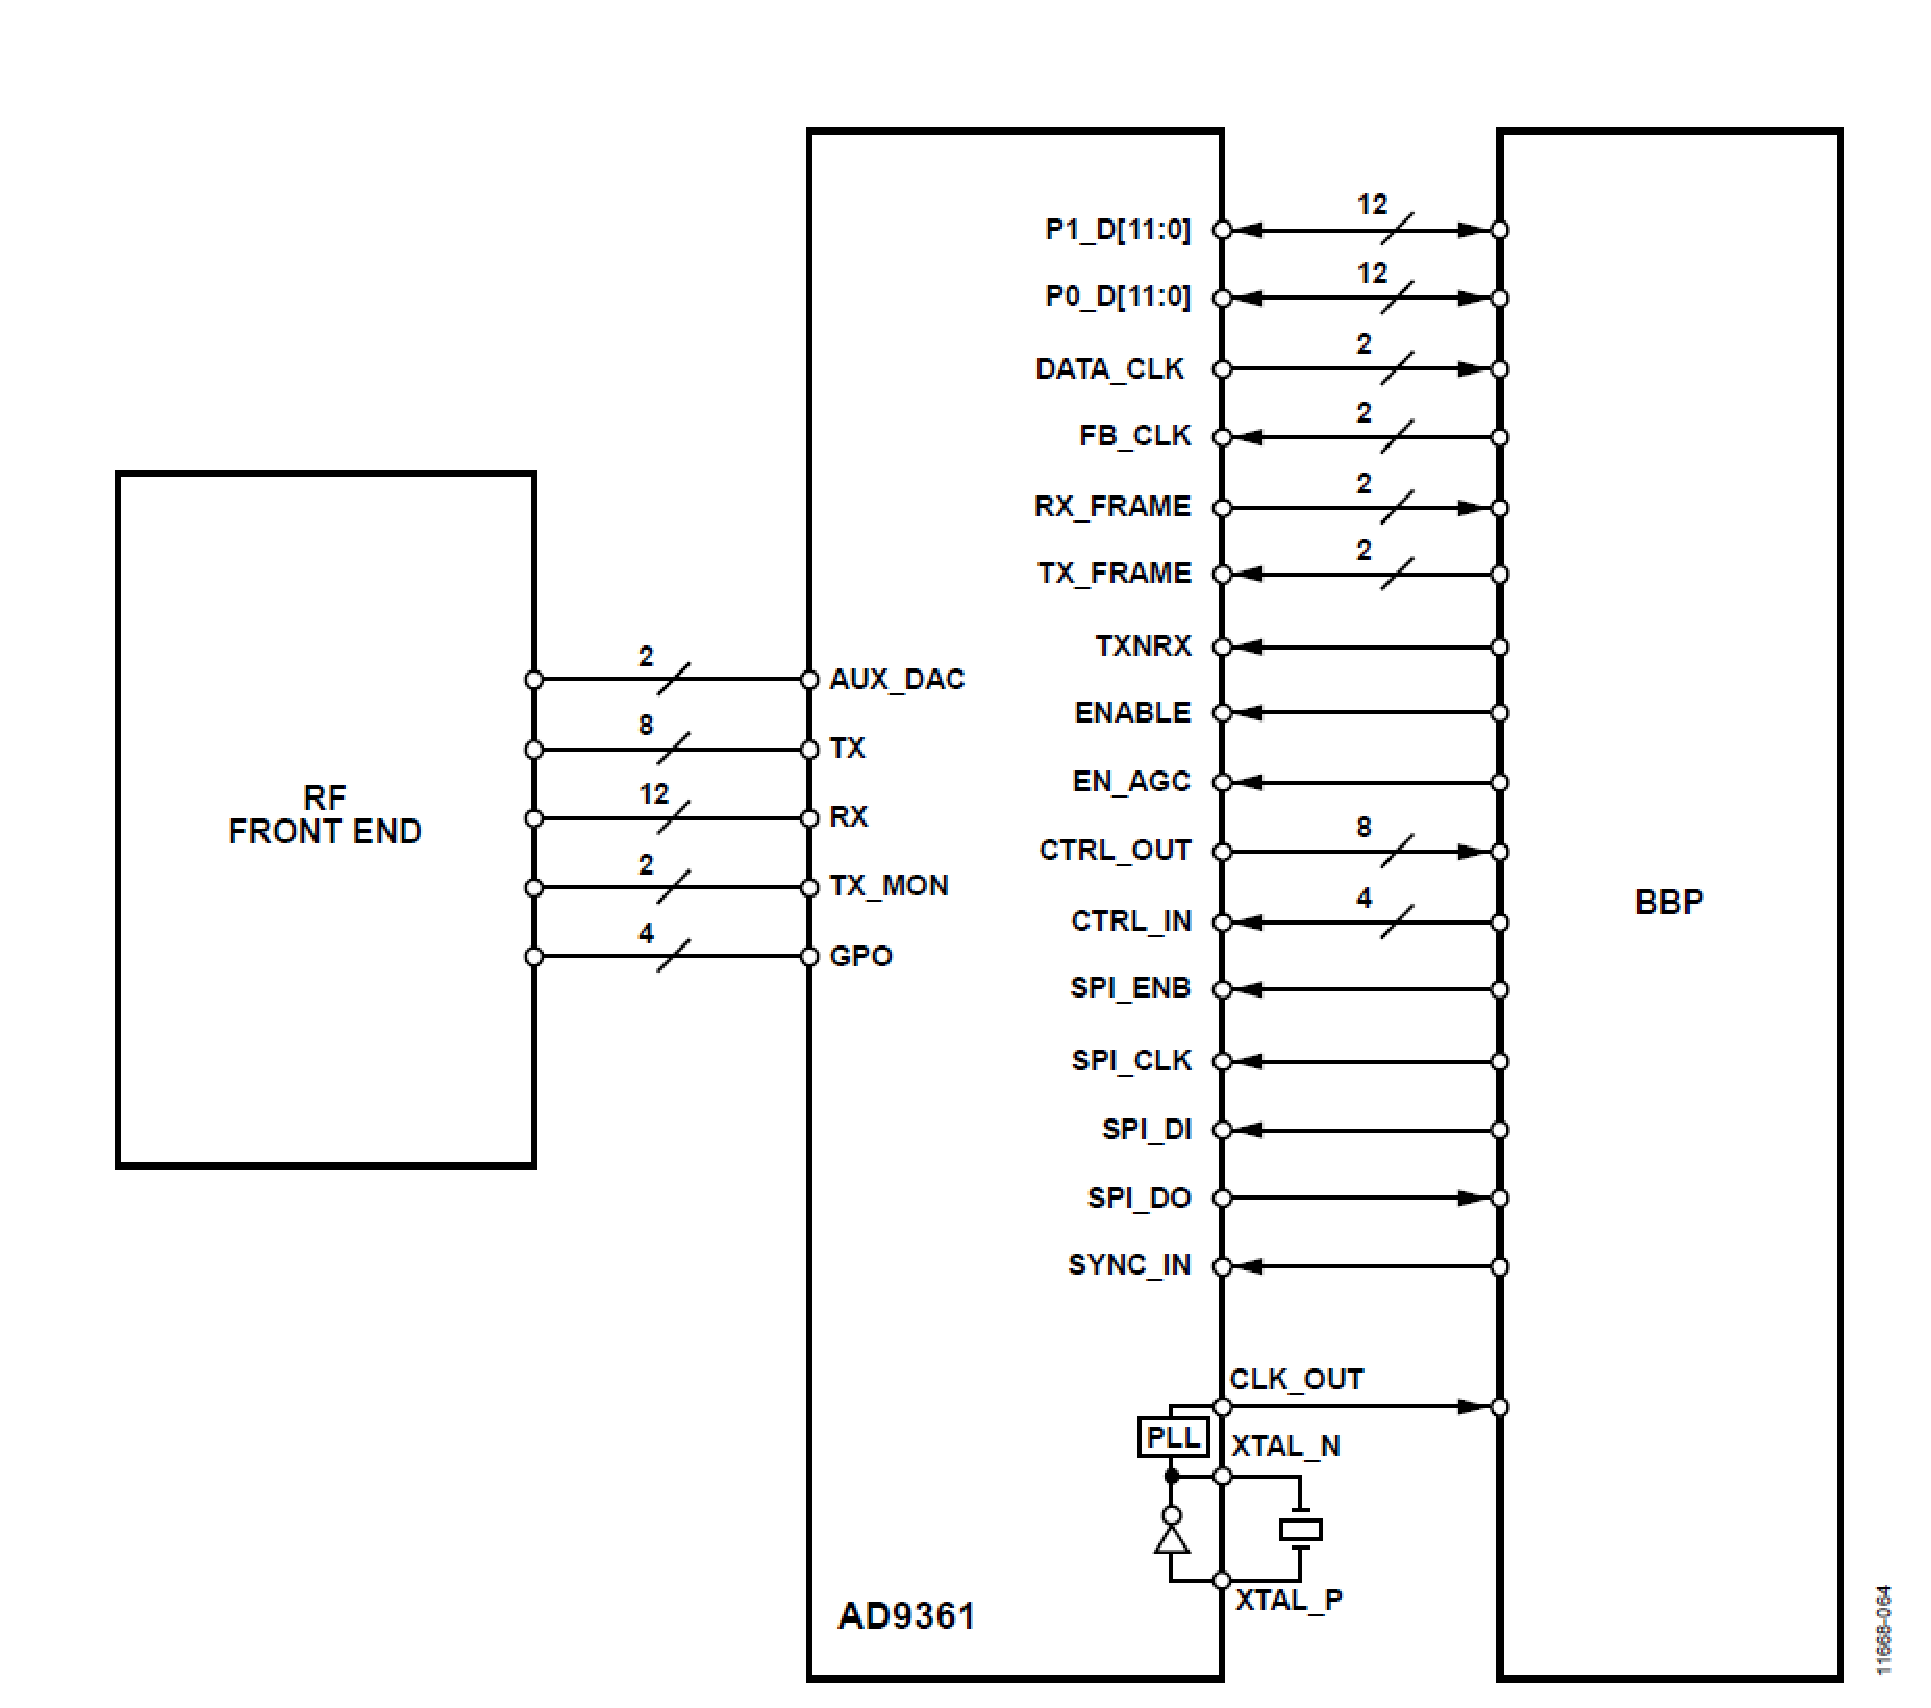
\includegraphics[width=0.65\textwidth]{./figures/ad9361_digital_interface}
    \caption{ AD9361 Digital Data Interface
    \label{fig:ad9361diginterface}}
\end{figure}

\subsection{Uplink Scheme}

During the study item phase of LTE, alternatives for the optimum uplink transmission
scheme were investigated. While OFDMA is seen optimum to fulfill the LTE
requirements in downlink, OFDMA properties are less favorable for the uplink. This is
mainly due to weaker peak-to-average power ratio (PAPR) properties of an OFDMA
signal, resulting in worse uplink coverage and challenges in power amplifier design for
battery operated handset, as it requires very linear power amplifiers.\\

Thus, the LTE uplink transmission scheme for FDD and TDD mode is based on SC-
FDMA (Single Carrier Frequency Division Multiple Access) with cyclic prefix. SCFDMA
signals have better PAPR properties compared to an OFDMA signal. This was
one of the main reasons for selecting SC-FDMA as LTE uplink access scheme. The
PAPR characteristics are important for cost-effective design of UE power amplifiers.
Still, SC-FDMA signal processing has some similarities with OFDMA signal processing,
so parameterization of downlink and uplink can be harmonized.\\

There are different possibilities how to generate an SC-FDMA signal. DFT-spread-
OFDM (DFT-s-OFDM) has been selected for E-UTRA which can be seen in figure X. For
DFT-s-OFDM, a size-M DFT is first applied to a block of M modulation
symbols. QPSK, 16QAM and 64QAM are used as uplink E-UTRA modulation
schemes, the latter being optional for the UE. The DFT transforms the modulation
symbols into the frequency domain. The result is mapped onto the available number
of subcarriers. For LTE Release 8 uplink, only localized transmission on consecutive
subcarriers is allowed. An N-point IFFT where N>M is then performed as in OFDM,
followed by addition of the cyclic prefix and parallel to serial conversion.

%figura uplink
\begin{figure}[htbp]
    \centering
    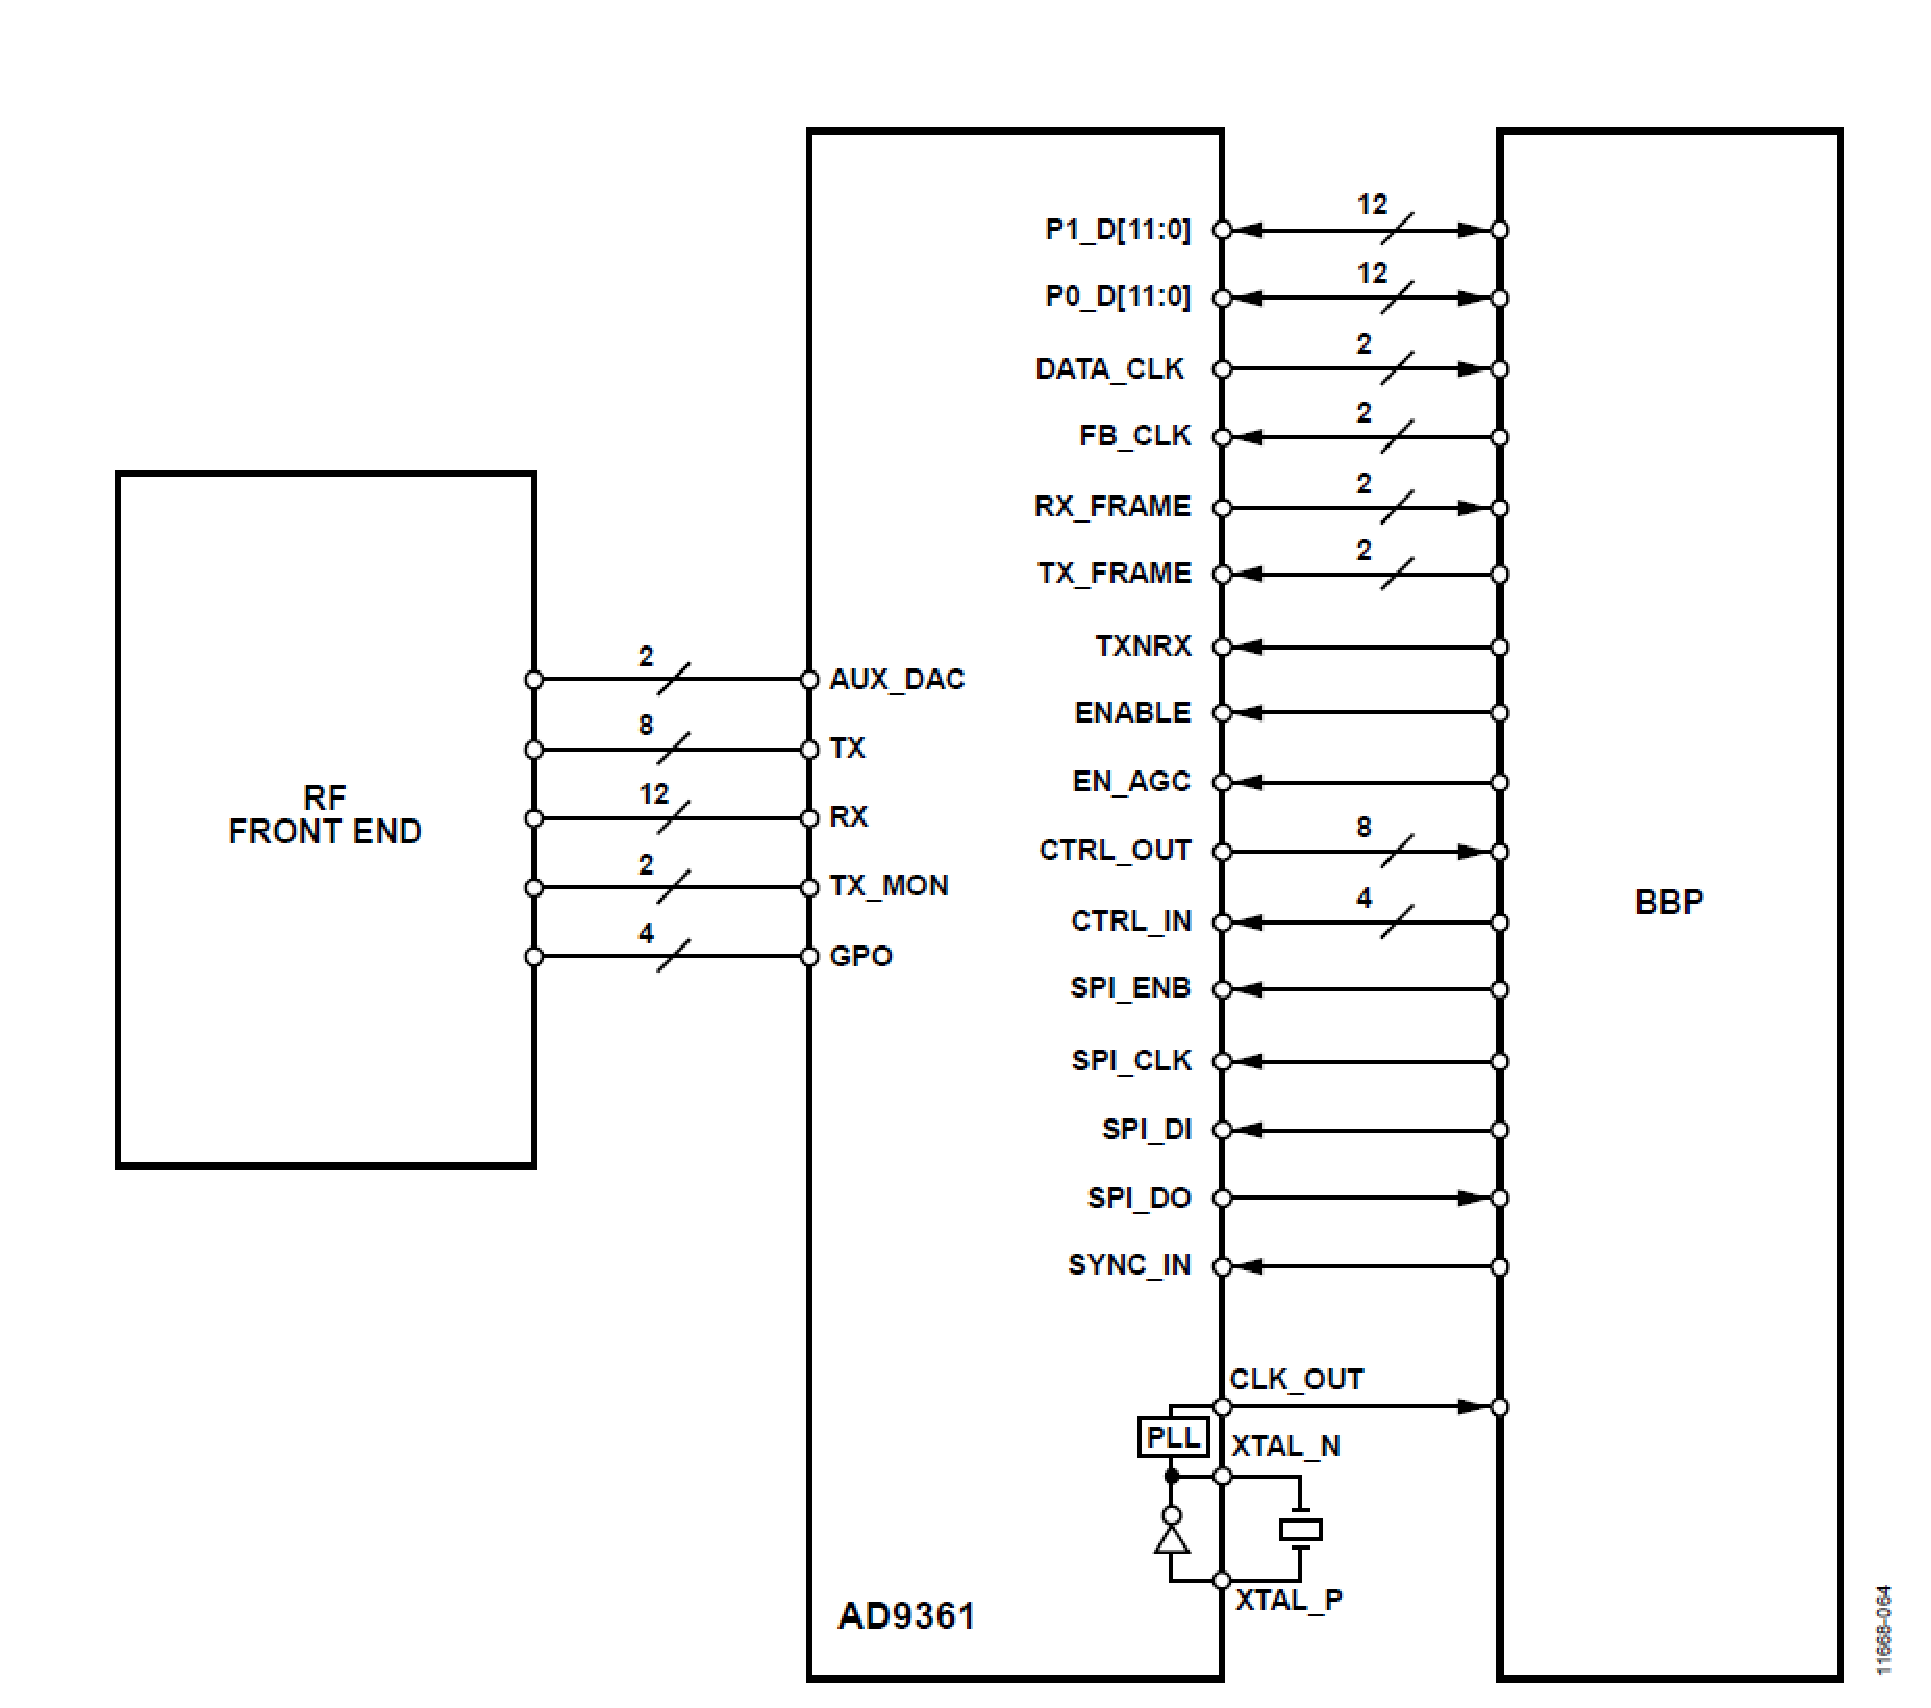
\includegraphics[width=0.65\textwidth]{./figures/ad9361_digital_interface}
    \caption{ AD9361 Digital Data Interface
    \label{fig:ad9361diginterface}}
\end{figure}
